\documentclass{beamer}
\hypersetup{unicode}
\usepackage[utf8]{inputenc}
\usepackage[croatian]{babel}
\usepackage{csquotes}
\MakeOuterQuote{"}
\usepackage{thmtools}

\declaretheorem{teorem}
\declaretheorem[style=remark, sibling=teorem]{primjer}
\declaretheorem[style=remark, sibling=teorem]{napomena}
\declaretheorem[style=definition, sibling=teorem]{definicija}

\usepackage[style=authoryear]{biblatex}
\addbibresource{literatura.bib}
\usepackage{tikz}

% manage colors: https://www.r-bloggers.com/2011/11/create-your-own-beamer-template/
% and https://ramblingacademic.com/2015/12/08/how-to-quickly-overhaul-beamer-colors/

\usetikzlibrary{arrows}
\newcommand{\midarrow}{\tikz \draw[-triangle 90] (0,0) -- +(.1,0);}

\definecolor{seagreen}{HTML}{21b2aa}
\definecolor{magenta}{HTML}{b2217f}
\definecolor{gold}{HTML}{ca9520}
\definecolor{red}{HTML}{da272f}
\definecolor{blue}{HTML}{4682b4}
\definecolor{purple}{HTML}{a65cef}

\definecolor{white}{HTML}{ffffff}
\definecolor{dwhite}{HTML}{eeeeee}
\definecolor{black}{HTML}{000000}
\definecolor{lblack}{HTML}{222222}

\colorlet{bgmain}{seagreen}
\colorlet{bgsec}{magenta}
\colorlet{bgter}{gold}
\colorlet{fgmain}{black}
\colorlet{fgsec}{lblack}

\usetheme{Madrid}
\usecolortheme{orchid}
% \useinnertheme{rounded}

\setbeamercolor{titlelike}{parent=structure, bg=seagreen, fg=white}
\setbeamercolor{palette primary}{bg=magenta, fg=white}
\setbeamercolor{palette secondary}{bg=magenta, fg=white}
\setbeamercolor{palette tertiary}{bg=magenta, fg=white}
\setbeamercolor{palette quaternary}{bg=magenta, fg=white}
\setbeamercolor{structure}{bg=white, fg=magenta} % itemize, enumerate, etc
\setbeamercolor{section in toc}{fg=black, bg=lblack} % TOC sections
\setbeamercolor{frametitle}{fg=white, bg=seagreen}

\setbeamercolor{block title}{fg=white, bg=seagreen}
% \setbeamercolor{block body}{bg=white, fg=white}

% Override palette coloring with secondary
\setbeamercolor{subsection in head/foot}{bg=seagreen,fg=white}



\title[Zadaća iz $LaTeX$a --- Beamer]{Treća zadaća iz $LaTeX$a}
\subtitle{Matematički softver}
\author{Luka Šimek}
\institute[PMF--MO]{Prirodoslovno-matematički fakultet --- Matematički odsjek\\Sveučilište u Zagrebu}
\date{\today}

\begin{document}

\begin{frame}[plain]
\titlepage
\end{frame}

\begin{frame}{Sadržaj}
\tableofcontents
\end{frame}

\section{Uvod}
\begin{frame}{Uvod --- definicija}
\begin{columns}[t]

\column{.4\textwidth}
\begin{definicija}
\emph{Slobodna grupa} $F = \langle S \rangle$ generirana skupom $S$ je grupa svih riječi sa znakovima iz $S$. 
\end{definicija}



\column{.3\textwidth}
\begin{napomena}
Elemente $S$ shvaćamo formalno, odnosno dvije riječi u $F$ su jednake samo ako to proizlazi iz aksioma grupe.
\end{napomena}


\end{columns}

\end{frame}

\section{Primjer}
\begin{frame}{Primjer slobodne grupe}
\onslide<1-> \begin{block}{Slobodna grupa reda $2$}
Slobodna grupa reda $2$ je do na izomorfizam jednaka $F_2 = \langle A, U\rangle $. Njome možemo (više u~\cite{conway}) prikazivati obilaske zatvorenih rubova. $A$ dolazi od eng.\ $\textsl{\textbf<1>{a}cross}$, $U$ od $\textsl{\textbf<1>{u}p}$.
\end{block}

\onslide<2->\begin{figure}[hb]
\centering
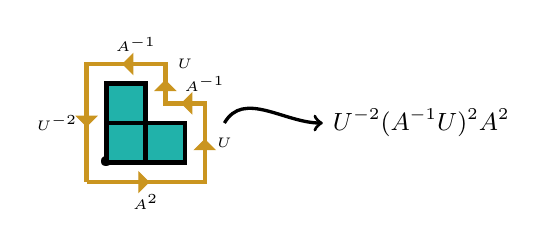
\begin{tikzpicture}

\node[minimum width=1cm] at (0,0) {\textbullet};
\draw[ultra thick, fill = seagreen] (0,0)rectangle(1/2,1/2);
\draw[ultra thick, fill = seagreen] (0,1/2)rectangle(1/2,1);
\draw[ultra thick, fill = seagreen] (1/2,0)rectangle(1,1/2);


%https://www.latex4technics.com/?note=29EJ
\begin{scope}[ultra thick, gold, every node/.style={sloped,allow upside down}]
\draw(-1/4,-1/4)--node {\midarrow}(5/4,-1/4)
--node {\midarrow}(5/4,1/2+1/4)
--node {\midarrow}(5/4-1/2,1/2+1/4)
--node {\midarrow}(5/4-1/2,1/2+3/4)
--node {\midarrow}(5/4-1/2-1/2-2/4,1/2+3/4)
--node {\midarrow}(-1/4,-1/4) ;
\end{scope}

\node at (1/2,-1/2) {\tiny $A^2$};
\node at (1+1/2,1/4) {\tiny $U$};
\node at (5/4,1) {\tiny $A^{-1}$};
\node at (5/4-1/4,1+1/4) {\tiny $U$};
\node at (1/2-1/8,1+1/2) {\tiny $A^{-1}$};
\node at (-2/4-1/8,1/2) {\tiny $U^{-2}$};

\node at (4,1/2) {\small $U^{-2}(A^{-1}U)^2A^2$};
\draw[very thick, ->] (1+1/2,1/2) to[out=60,in=180] (2+3/4,1/2);

\end{tikzpicture}
\caption{primjer poistovjećenja (orijentiranog) ruba i riječi iz $F_2$}
\label{}
\end{figure}
\end{frame}



\begin{frame}[t]{Literatura}
\printbibliography
\end{frame}
\end{document}


